% !TEX root = ../../main.tex

Nella sezione seguente si presenta da dove sono stati reperiti i dati di partenza e quali scelte sono state fatte nella costruzione di serie di estremi di temperatura giornalieri.

\subsection{Disponibilità e qualità di dati e metadati}
Al fine di preparare il dataset delle climatologie si è reso necessario raccogliere, controllare e combinare i dati rilevati dalle stazioni meteorologiche distribuite sul territorio italiano e nelle zone limitrofe all'arco alpino, in modo da avere a disposizione serie di valori minimi e massimi giornalieri di temperatura (si userà in seguito anche il termine ``estremi'' di temperatura). Tale operazione è risultata particolarmente complessa, per le misure effettuate nel trentennio 1991--2020, a causa della frammentarietà e disomogeneità delle sorgenti di dati, attribuibili a tre ragioni principali. Innanzitutto, vi è un elevato numero di soggetti coinvolti nella gestione delle principali reti di rilevazione meteorologica e dei dati da esse derivanti. Questo fenomeno ha avuto origine nel trasferimento di competenze del Servizio Idrografico e Mareografico Nazionale (SIMN) a centri funzionali, Dipartimento di Protezione Civile (DPC) e Agenzie Regionali per la Protezione dell'Ambiente (ARPA)~\cite{InquadramentoStoricoMonitoraggio} avvenuto all'inizio degli anni 2000. Tali enti e agenzie non seguono un protocollo nazionale che omogenizzi i criteri di gestione della rete e dell'elaborazione e distribuzione dei dati, per cui persino raccogliere i dataset risulta un problema non banale, avendo a che fare con più di 20 tra archivi regionali e provinciali con interfacce per l'accesso ai dati di varia efficacia. In secondo luogo, dalla fine degli anni '80 vi è stata una progressiva diffusione dei sistemi di rilevamento automatico, accompagnata dalla dismissione di quelli meccanici. Questo cambiamento ha introdotto significative disomogeneità nelle serie temporali e spesso ha portato al loro troncamento, laddove la stazione di riferimento non sia stata rimpiazzata. Infine si riscontra una generale carenza di documentazione relativa alle stazioni stesse: di norma si trovano liste di nominativi di stazione, posizioni e quote (non di rado imprecise), mentre sono pochi gli enti che forniscono uno storico delle modifiche apportate alle stazioni (eventuali ricollocamenti, cambiamenti nelle tipologie di sensori, ecc.).

Nell'ambito di questo lavoro di tesi mi sono concentrato sulle regioni del centro-nord Italia, fino a Toscana, Umbria e Marche comprese, e sulle zone circostanti l'arco alpino (fino a \qty{200}{\kilo\meter} nei territori di Francia, Svizzera, Austria e Slovenia).

La maggior parte dei dati raccolti sono stati forniti come aggregazioni a livello giornaliero, solo in poche situazioni si è fatto ricorso ai dati grezzi sub-giornalieri. Da un'analisi preliminare è risultato evidente che ogni rete o gestore di dataset utilizza un proprio criterio nel calcolare tali stime a partire dai dati rilevati dai sensori. In particolare, si sono incontrate scelte differenti riguardo i seguenti ambiti:

\begin{itemize}
  \item
    definizione di ``giornata di misura'': in alcuni casi inizia alle 09:00 del giorno dichiarato (approccio dell'ex Servizio Idrografico), in altri alle 00:00 (approccio moderno);
  \item
    timezone delle date: vengono utilizzati GMT o CET;
  \item
    aggregazione dei dati sub-giornalieri: vengono forniti gli estremi assoluti delle temperature rilevate nel corso della giornata (in linea con quanto cercato per la tesi) o gli estremi delle medie orarie (sempre distanti al più qualche decimo di grado dagli estremi assoluti e sempre ``meno estremi'' rispetto a essi).
\end{itemize}

La disponibilità temporale e spaziale delle serie nei singoli dataset infine risulta essere perlopiù incompleta: ad esempio dataset nazionali come SCIA, quello del DPC e del CNR-ISAC risultano essere incompleti nei termini della distribuzione spaziale delle serie, mentre quelli regionali non registrano le misure antecedenti al passaggio di competenze citato in precedenza.

La presenza delle problematiche illustrate e la necessità di serie giornaliere il più possibile complete e consistenti sotto il profilo sia temporale che spaziale hanno reso necessaria l'elaborazione di procedure adeguate di merging dei singoli dataset e saranno presentate nella sezione~\ref{ch:merging}.

\subsection{Sorgenti utilizzate}\label{ch:sources}
Nella tabella~\ref{tab:quick-datasets} sono elencati i dataset impiegati per il lavoro. In appendice la figura~\ref{fig:regional-monthly} mostra la disponibilità di serie a scala mensile regione per regione.

\begin{table}[ht]
  \centering
  \begin{threeparttable}
    \caption{Elenco dei dataset utilizzati}\label{tab:quick-datasets}
    \begin{tabular}{l l l}
      \toprule
      Nome & Copertura & Disponibilità\tnote{*} \\
      \midrule
      SCIA & Italia & 2563 \\
      DPC & Italia & 2201 \\
      CNR-ISAC & Italia & 280 \\
      ARPA Piemonte & Regione & 326 \\
      ARPA Lombardia & Regione & 255 \\
      ARPA Veneto & Regione & 255 \\
      MeteoTrentino & Provincia (Trento) & 194 \\
      CIVIS Bolzano & Provincia & 66 \\
      ARPA FVG/OSMER & Regione & 57 \\
      ARPAL & Regione (Liguria) & 188 \\
      SIR Toscana & Regione & 441 \\
      Dext3r & Regione (Emilia-Romagna) & 623 \\
      ARPAM & Regione (Marche) & 157 \\
      ARPA Umbria & Regione & 75 \\
      MeteoFrance & Francia & 2196 \\
      GeoSphere Austria & Austria & 625 \\
      ARSO Meteo & Slovenia & 570 \\
      Agrometeo CH & Svizzera & 196 \\
      WSL & Svizzera & 223 \\
      SwissMetNet & Svizzera & 857 \\
      \bottomrule
    \end{tabular}
    \begin{tablenotes}
    \item[*] \small Numero di stazioni presenti nel dataset come reperito. Si calcolano solo quelle nel territorio in esame.
    \end{tablenotes}
  \end{threeparttable}
\end{table}

A livello qualitativo si è constatato che:

\begin{itemize}
  \item
    i dataset regionali sono i meglio forniti in quanto a dati recenti (post-2000) e qualità delle anagrafiche delle stazioni;
  \item
    SCIA è ben fornito di dati storici (pre-2000), mentre quelli recenti sono incompleti; le stazioni sono spesso collocate in maniera poco accurata. Inoltre, pur essendo passate da un'operazione di \emph{quality check} alcune serie contengono errori significativi (in particolare le sinottiche);
  \item
    CNR-ISAC fornisce qualche centinaio di serie lunghe già omogeneizzate;
  \item
    DPC registra serie spesso non presenti negli altri dataset, tuttavia fornisce gli estremi giornalieri delle medie orarie invece che gli estremi assoluti e le stazioni sono spesso collocate in maniera poco accurata.
\end{itemize}

\subsection{Merging}\label{ch:merging}
La procedura di merging ha per scopo la combinazione delle varie sequenze di dati in serie rappresentative della collocazione geografica delle stazioni di rilevazione. Nell'elaborarla si è prestata particolare attenzione a due questioni: l'unione delle sequenze duplicate o ridondanti (merging ``orizzontale'') e l'aggregazione di sequenze rappresentative di una stessa località geografica ma provenienti da stazioni o sensori diversi (merging ``verticale''). Né il primo né il secondo problema hanno avuto soluzione immediata a causa della mancanza di codici di identificazione univoci, delle inaccuratezze sul collocamento geografico delle stazioni e di varie incongruenze nella registrazione dei valori di temperatura. La carenza di informazioni ha reso impossibile, in diversi casi, determinare con assoluta certezza se un insieme di sequenze provenisse dalla stessa stazione o meno: per tale ragione il criterio di merging è formulato in termini di rappresentatività geografica delle serie, piuttosto che di identità delle stazioni. In ogni caso si è cercato di mantenere separate le sequenze provenienti da stazioni diverse, integrando le situazioni dubbie solo nel caso in cui fosse ragionevole credere di avere a che fare con stazioni distanti al più qualche centinaio di metri in un contesto urbano o pianeggiante.

Il procedimento definitivo si articola in due fasi: l'identificazione delle sequenze facenti parte della stessa serie e l'unione di queste in singole serie.

\subsubsection{Identificazione delle serie}
\begin{figure}[ht]
  \centering
  \includegraphics[width=\textwidth]{images/creazione_dataset/raccolta_dati/reggio_series_osm.pdf}
  \caption{Sequenze originali nella zona di Reggio Emilia. Si possono notare quattro raggruppamenti principali più una stazione apparentemente isolata. Non tutte le sequenze sono etichettate per rendere più fruibile l'immagine. Mappa di base fornita da Esri~\autocite{esriWorldTopographicMap2013}.}\label{fig:reggio-osm}
\end{figure}
\begin{figure}[ht]
  \centering
  \input{images/creazione_dataset/raccolta_dati/reggio_series_plot.tex}
  \caption{Estratto delle sequenze introdotte nella figura~\ref{fig:reggio-osm}, scelte tra quelle collocate nella città di Reggio Emilia. Sembrerebbero rappresentare una stazione ricollocata nel 2007 o nel 2008, tuttavia ogni sorgente dà una versione differente. Alcune hanno eliminato dei dati (buchi nella sequenza) probabilmente a causa di un controllo qualità con esito negativo.}\label{fig:reggio-plot}
\end{figure}
Se si considerano le sequenze recuperate dai vari dataset come i vertici di un grafo le cui connessioni sono costituite dalla relazione ``fanno parte della stessa serie'' (da qui in poi ``\emph{match}''), il problema in esame ha come soluzione le componenti connesse del suddetto grafo. Questo approccio consente di definire una relazione di connessione, che in generale potrebbe essere molto articolata, in maniera non necessariamente esaustiva, dal momento che automatizza il raggruppamento di più sequenze anche quando non ci sono \emph{match} tra tutte le componenti e ogni altra. Un esempio di grafo fatto in questo modo è presentato in figura~\ref{fig:reggio-graph}.

Idealmente, per individuare un \emph{match}, basterebbe controllare l'uguaglianza delle sequenze di dati attribuite ai sensori nei vari dataset, o degli identificativi univoci delle stazioni, oppure la coincidenza o prossimità delle loro posizioni. Non è però questo il caso per i cataloghi a disposizione. In particolare, i problemi riscontrati nell'effettuare \emph{matching} tra serie inter- e intra-dataset sono legati a:

\begin{itemize}
  \item inaccuratezza nel collocamento spaziale legata alla precisione numerica del dato registrato (generalmente accade per le stazioni meno recenti) e a conversioni del sistema di riferimento (si osservi, ad esempio, la figura~\ref{fig:reggio-osm});
  \item prossimità di stazioni differenti, come avviene in particolare nei contesti cittadini o in compresenza di reti diverse (ad esempio DPC, regionali, e servizi agrometeorologici);
  \item differenze nelle anagrafiche: dal semplice utilizzo di caratteri accentati o simboli all'impiego di nomi di località differenti;
  \item assenza o incompletezza dei codici identificativi univoci delle stazioni;
  \item differenze nella stima degli estremi giornalieri: estremi delle medie orarie o estremi assoluti giornalieri;
  \item presenza di serie già integrate con i dati di altre;
  \item differenti definizioni di ``giornata meteorologica'' come esposto in precedenza.
  \item presenza di serie già integrate con i dati di altre o, viceversa, incomplete (si veda la figura~\ref{fig:reggio-plot}).
\end{itemize}

Queste osservazioni e la generale mancanza di una documentazione approfondita dei cataloghi che spieghi i criteri di raccolta dati, impongono l'elaborazione di metodi empirici e parametrici (adattabili quindi a combinazioni di network diversi) per determinare i \emph{match} tra le sequenze. Si è scelto di utilizzare per la classificazione un approccio ad albero decisionale, che porta alla dichiarazione di \emph{match} avvenuto sottoponendo le coppie candidate a una successione di test di confronto a esito binario su parametri scelti in maniera ponderata. Partendo da considerazioni banali (due sequenze della stessa serie dovrebbero avere dati uguali o ``simili'', nomi simili ed essere ragionevolmente vicine) e confrontando dati e metadati per via grafica e tabulare si è giunti alla scelta del seguente set di parametri:

\begin{itemize}
  \item
    media delle differenze tra stime giornaliere, medie mensili e climatologie mensili prese con e senza valore assoluto;
  \item
    distanza sul piano tra le posizioni dichiarate;
  \item
    differenza tra le quote dichiarate;
  \item
    somiglianza tra nomi di stazione secondo l'algoritmo Jaro-Winkler;
  \item
    \(\mathrm{f}_0\): percentuale di stime giornaliere identiche al decimo di grado sull'insieme dei giorni di misura comuni alle sequenze;
  \item
    \(\mathrm{b}\): media dei segni delle differenze tra stime giornaliere diverse da 0 (permette di capire in quanta parte le misure di una stazione sono consistentemente maggiori o minori di quelle dell'altra);
  \item
    \(\mathrm{n_d}\): numero di giorni in cui entrambe le serie hanno misure valide.
\end{itemize}

\begin{figure}[ht]
  \centering
  \makebox[\textwidth][c]{\includegraphics[width=1.4\textwidth]{images/creazione_dataset/raccolta_dati/reggio_series_graph.pdf}}
  % \input{images/creazione_dataset/raccolta_dati/reggio_series_graph}
  % \includegraphics[width=\textwidth]{images/creazione_dataset/raccolta_dati/reggio_series_graph_p.pdf}
  \caption{Grafo delle sequenze presentate nella figura~\ref{fig:reggio-osm}. Si può notare come la varietà di nomi forniti in anagrafica (riportati sulle etichette), l'estensione dei possibili \(\mathrm{f}_0\) e delle distanze a cui sono collocate rendono la procedura di identificazione dei \emph{match} non banale e difficilmente esaustiva.}\label{fig:reggio-graph}
\end{figure}

Nell'elaborazione del dataset italiano i \emph{match} sono stati cercati nell'insieme delle stazioni distanti al più \(15\:\mathrm{km}\) le une dalle altre secondo le posizioni dichiarate. Tale soglia è dovuta alle imprecisioni talvolta molto importanti nelle anagrafiche. Sono stati calcolati i parametri introducendo nelle sequenze offset di -1, 0 e +1 giorni, per trovare \emph{match} anche nelle situazioni in cui le stime sono state attribuite alla giornata precedente o successiva a quella dichiarata (cosa che capita ad esempio quando le definizioni di giornata meteorologica sono diverse).

Per ogni accoppiamento di dataset o di network di stazioni si sono fissati empiricamente dei valori di soglia per i parametri sopra elencati da utilizzare nei test di confronto dell'albero decisionale. Si è partiti dalle seguenti considerazioni:

\begin{itemize}
  \item
    valori rilevanti di \(\mathrm{f}_0\) (\(> \qty{15}{\percent}\)) a fronte di un numero significativo di giorni in comune (\(\mathrm{n_d} > 100\)) dovrebbero indicare un match ``orizzontale'';
  \item
    distanze ridotte (\(< 500\:\mathrm{m}\)) o valori di somiglianza tra anagrafiche alti (\(> \qty{90}{\percent}\)) potrebbero indicare sia match ``orizzontali'' che ``verticali'';
  \item
    valori rilevanti di \(\mathrm{f}_0\) associati a valori estremi di \(|\mathrm{b}|\) (\(\ge 0.8\)) e di segno discorde per le sequenze di minime e massime potrebbero indicare \emph{match} tra serie di estremi assoluti e di estremi delle medie orarie.
\end{itemize}

Tali criteri sono stati adattati e integrati a seconda dei casi confrontando le analisi dei candidati match in tabelle. La bontà delle soglie scelte è stata valutata esaminando manualmente un campione rappresentativo dei risultati di ogni passaggio del merging controllando i grafici delle differenze tra valori delle stazioni accoppiate, le posizioni in anagrafica su Google Earth e tutti i casi in cui la media delle differenze fosse maggiore di \(\qty{0.5}{\degreeCelsius}\).

In alcune situazioni le soglie individuate non sono risultate sufficienti a stabilire i \emph{match} alla perfezione: si sono dovute fare integrazioni manuali sia per dichiarare situazioni di \emph{match} che per negare quelle trovate dalla procedura automatica.

\subsubsection{Unione delle sequenze}
L'unione delle sequenze consiste nella combinazione di dati e metadati delle sequenze che compongono ogni serie allo scopo di compensare eventuali carenze. L'operazione viene effettuata integrando con gli elementi di ciascuna componente del grafo, una alla volta, una serie master. Ciò richiede di stabilire criteri di preferenza e di accettabilità per l'unione sia dei metadati che dei dati.

Per quanto riguarda l'ordine di unione, tenendo conto delle osservazioni generali esposte nella sezione~\ref{ch:sources}, si è generalmente scelto di preferire i metadati delle agenzie regionali/provinciali a quelli dei dataset nazionali; per i dati invece si sono prese come riferimento le sequenze omogeneizzate ISAC-CNR, seguite in ordine da quelle delle agenzie regionali/provinciali, quelle di SCIA e infine quelle del DPC. Come secondo criterio d'ordine, usato nei casi di pareggio del primo, si è presa la lontananza temporale dei dati forniti, con priorità data alle sequenze più recenti (che hanno generalmente metadati più accurati), nell'ottica che il database possa essere aggiornato in maniera continuativa e riflettere la situazione attuale delle stazioni italiane.

Per quanto riguarda il protocollo d'integrazione delle stime giornaliere, si è scelto di aggiungere alla sequenza master i valori delle sequenze integranti prese una alla volta nell'ordine stabilito dai criteri di preferenza, a condizione che i contributi di ogni sequenza integrante superino i due anni.
L'inserimento avviene dopo aver sommato ai dati grezzi della serie integrante una correzione modellizzata sulle anomalie rispetto alla master in funzione del giorno dell'anno. Tale modello viene scelto tra una serie di Fourier troncata al terzo ordine, la media o lo zero, in base alla dimensione e alla distribuzione del campione di anomalie:

\begin{align*}
  T_m(d) &= T_i(d) + \Delta T_{i,m}(d) \\
  \Delta T_{i,m}(d) &\sim
  \begin{cases}
    \frac{a_0}{2} + \sum^3_{n=1} a_n \cos( 2\pi n t(d)) + b_n\sin(2\pi n t(d)) & \text{se } \mathcal{I}_{i,m} \ge 8 \\
    \frac{a_0}{2} & \text{se } 2 \le \mathcal{I}_{i,m} < 8 \\
    \qty{0}{\degreeCelsius} & \text{altrimenti} \\
  \end{cases}
\end{align*}

dove \(d\) è una data, \(t(d)\) indica il numero di giorno dell'anno di \(d\) normalizzato rispetto alla lunghezza dell'anno di riferimento e \(\mathcal{I}_{i,m}\) il numero di diversi mesi dell'anno per cui si hanno almeno 20 anomalie valide. La validità di un'anomalia per un dato giorno e la sua conseguente inclusione nel sample del modello sono determinate dalla compresenza di dati di temperatura nella sequenza master e in quella integrante e dall'assenza di incongruenze dovute a errori palesi (dev'essere \(|T_x(d)| < \qty{50}{\degreeCelsius}\) e \(|\Delta T_{m,i}(d)| < \qty{10}{\degreeCelsius}\)). Per evitare di introdurre correzioni superflue i coefficienti di correzione vengono azzerati a posteriori se \(|a_0/2| = |\langle \Delta T_{m,i} \rangle| < \qty{0.1}{\degreeCelsius}\) e \(|a_i|, |b_i| < \qty{0.2}{\degreeCelsius}\), mentre se \(|\langle \Delta T_{m,i} \rangle| > \qty{1}{\degreeCelsius}\) l'unione viene saltata e la serie integrante scartata. Il merging, infine, avviene in maniera simmetrica per le serie di massime e di minime: se una delle due non soddisfa i criteri di validità, entrambe le sequenze vengono scartate.

Le serie scartate in fase di merging vanno perdute: si è notato, lavorandoci, che spesso sono serie con errori evidenti. Lo scarto inoltre è stato utilizzato come criterio di valutazione a ritroso dei parametri di soglia scelti per il merging, e in vari casi ha portato a ridefinire manualmente alcuni \emph{match}.

\subsubsection{Correzione delle anagrafiche}
È stata quindi effettuata una correzione delle informazioni spaziali ottenute nelle anagrafiche delle serie combinate, al fine di migliorare la qualità delle variabili su cui si basano i modelli di interpolazione geostatistica. Dato l'elevato numero di stazioni ci si è concentrati su un sottoinsieme di casi sospetti, identificati confrontando le quote dichiarate in anagrafica con quelle del DEM a risoluzione \qty{30}{\meter} Copernicus GLO 30~\cite{europeanspaceagencyCopernicusGlobalEuropean2022} ed esaminando tutti i casi di discrepanze superiori a \qty{10}{\meter} verticali. Si è quindi cercato, tramite immagini satellitari e fotografie (reperite tramite Google Earth, Google Street View e raccolte di anagrafiche di terze parti~\cite{associazionelineameteoStazioniReteLinea}), di determinare latitudine, longitudine e quote esatte delle stazioni. L'operazione è risultata più semplice, naturalmente, per stazioni moderne (di cui spesso si riesce a trovare traccia nelle fotografie); in tutti i casi analizzati si è tenuto traccia nel database delle modifiche apportate. La figura~\ref{fig:corrections-deltas} mostra le distribuzioni delle correzioni apportate alle posizioni e alle quote, che in circa la metà dei casi sono molto significative per le quote (\(\Delta \mathrm{H} > \qty{50}{\meter}\)).
% La tabella~\ref{tab:n-corrections} invece riporta il numero di correzioni apportate.

\begin{figure}[ht]
  \centering
  \input{images/creazione_dataset/correzioni/corrections_deltas.tex}
  \caption{Distribuzione delle correzioni di posizione e quota. Sono stati inclusi solo i casi in cui la correzione è superiore a \qty{10}{\meter}.}\label{fig:corrections-deltas}
\end{figure}

\subsubsection{Secondo merging}
Ultimo passaggio della procedura è un secondo merging effettuato esclusivamente all'interno del dataset ottenuto tramite i passaggi precedenti, al fine di eliminare eventuali duplicati rimasti. Effettuando la procedura di volta in volta tra un determinato dataset regionale e quelli nazionali infatti si possono perdere eventuali ridondanze tra i dataset regionali. Tale passaggio ha portato all'eliminazione di 66 serie, perlopiù provenienti da Dext3r e ARPAPiemonte.

\subsection{Risultati}\label{ch:results}
Si riportano di seguito alcune caratteristiche del dataset ottenuto tramite merging, per il trentennio 1991--2020. Tale dataset è, a questo punto del procedimento, un catalogo di stime degli estremi giornalieri di temperatura non controllati e non omogeneizzati, ma che rappresenta una base di partenza per la stima delle normali climatiche. Sono state considerate, nella presentazione che segue, soltanto le serie con almeno cinque anni di dati (anche non validi ai fini delle climatologie).

Nella tabella~\ref{tab:series-stats} si può vedere a confronto i numeri di serie disponibili che caratterizzano i dataset nazionali (limitandosi al territorio del centro-nord Italia: le serie estere sono escluse). Mentre SCIA rimane quello con più sequenze in termini assoluti (considerando l'intero dataset, compresi duplicati e serie antecedenti al 1991), le colonne ``Climatologie'' e ``Numero di mesi'' mostrano che le integrazioni di dati hanno portato a un incremento apprezzabile delle serie con i requisiti necessari a elaborare le climatologie nel trentennio 1991--2000 e in generale notevole dei dati a disposizione rispetto agli altri dataset.

\begin{table}[ht]
  \centering
  \begin{threeparttable}
    \caption{Serie nei dataset estesi.}\label{tab:series-stats}
    \scriptsize
    
\begin{tabular}{lrrrrr}
  \toprule
  Dataset & Densità [\unit{\kilo\meter^{-2}}] & Serie & Climatologie\tnote{*} \tnote{1} & Numero di mesi\tnote{*} \tnote{2} & Numero di dati\tnote{*} \tnote{3}\\
  \midrule
  merged & 0.016 & 2508 & 2357 & 524852 & 32134939\\
  SCIA & 0.016 & 2567 & 2008 & 382662 & 23641181\\
  ISAC & 0.002 & 280 & 271 & 81344 & 5014172\\
  DPC & 0.014 & 2205 & 1347 & 232210 & 14277744\\
  \bottomrule
\end{tabular}

    \begin{tablenotes}
    \item[\dag] Limitazione alle serie italiane.
    \item [*] Periodo 1991--2020.
    \item [1] Numero di serie con i requisiti minimi per calcolare le climatologie, ovvero cinque anni con mesi validi. Minimo tra temperature minime e massime.
    \item [2] Mesi con almeno venti giorni di misure e non più di quattro giorni consecutivi senza misure. Minimo tra temperature minime e massime.
    \item [3] Giorni con misure. Somma di minime e massime.
    \end{tablenotes}
  \end{threeparttable}
\end{table}

Nella figura~\ref{fig:merged-series} si può vedere la distribuzione spaziale delle serie ottenute tramite merging nel centro-nord Italia. A sinistra si vede che le serie che presentano le lacune più significative sono collocate in regioni specifiche, mentre a destra si nota dove SCIA ha le carenze maggiori nel trentennio considerato. Esclusa l'Emilia-Romagna, dove non si è fatto il merging con SCIA (salvo per le stazioni sinottiche), Lombardia, Toscana e Trentino-Alto Adige sono le regioni in cui l'integrazione con gli altri dataset (in particolar modo quelli regionali/provinciali) ha portato a un incremento significativo delle serie disponibili.
\begin{figure}[ht]
  \centering
  \includegraphics[width=\textwidth]{images/creazione_dataset/dataset/merged/spatial_availability.pdf}
  \caption{Distribuzione spaziale delle serie ottenute tramite merging nel centro-nord Italia. A sinistra la distribuzione di quelle che hanno la disponibilità di dati per calcolare delle climatologie. A destra le serie per cui esiste un \emph{match} con almeno una stazione di SCIA. Si trascuri l'Emilia-Romagna, dove SCIA è stato considerato in maniera parziale.}\label{fig:merged-series}
\end{figure}

La figura~\ref{fig:merged-timeseries} mette a confronto il numero di serie con mesi validi per il calcolo delle climatologie nei periodi pre- e post-1991. Nel periodo pre-1991 il nuovo dataset non offre un incremento significativo dei dati disponibili (del resto sono poche le serie regionali a dare contributi in questo periodo), mentre in quello successivo sì. In particolare SCIA mostra carenze importanti nell'ultimo decennio. In generale il numero di serie con assenza di disponibilità mensile risulta essere sempre poco rilevante rispetto al totale.
\begin{figure}[ht]
  \centering
  \input{images/creazione_dataset/dataset/monthly_availability.tex}
  \caption{Numero di serie con disponibilità mensile soddisfacente sul territorio del centro-nord Italia.}\label{fig:merged-timeseries}
\end{figure}

La figura~\ref{fig:merged-elevations} mostra la rappresentatività delle quote delle serie ottenute tramite merging e dei dataset nazionali sorgenti rispetto all'elevazione del territorio calcolata tramite un sample di \num{500000} punti del DEM~\cite{europeanspaceagencyCopernicusGlobalEuropean2022}. Il nuovo dataset tende a sottorappresentare le quote inferiori a \qty{300}{\meter} e a sovrarappresentare quelle fino a \qty{2000}{\meter}, anche se non in maniera irragionevole.
\begin{figure}[ht]
  \centering
  % Created by tikzDevice version 0.12.6 on 2025-04-07 21:10:49
% !TEX encoding = UTF-8 Unicode
\begin{tikzpicture}[x=1pt,y=1pt]
  \definecolor{fillColor}{RGB}{255,255,255}
  \path[use as bounding box,fill=fillColor] (0,0) rectangle (170.72, 88.20);
  \begin{scope}
    \path[clip] (  0.00,  0.00) rectangle (170.72, 88.20);
    \definecolor{drawColor}{RGB}{255,255,255}

    \path[draw=drawColor,line width= 0.6pt,line join=round,line cap=round,fill=fillColor] (  0.00,  0.00) rectangle (170.72, 88.20);
  \end{scope}
  \begin{scope}
    \path[clip] ( 44.69, 27.29) rectangle (165.22, 65.79);
    \definecolor{fillColor}{RGB}{255,255,255}

    \path[fill=fillColor] ( 44.69, 27.29) rectangle (165.22, 65.79);
    \definecolor{drawColor}{gray}{0.92}

    \path[draw=drawColor,line width= 0.3pt,line join=round] ( 44.69, 33.71) --
    (165.22, 33.71);

    \path[draw=drawColor,line width= 0.3pt,line join=round] ( 44.69, 43.07) --
    (165.22, 43.07);

    \path[draw=drawColor,line width= 0.3pt,line join=round] ( 44.69, 52.42) --
    (165.22, 52.42);

    \path[draw=drawColor,line width= 0.3pt,line join=round] ( 44.69, 61.77) --
    (165.22, 61.77);

    \path[draw=drawColor,line width= 0.3pt,line join=round] ( 64.58, 27.29) --
    ( 64.58, 65.79);

    \path[draw=drawColor,line width= 0.3pt,line join=round] ( 87.65, 27.29) --
    ( 87.65, 65.79);

    \path[draw=drawColor,line width= 0.3pt,line join=round] (110.72, 27.29) --
    (110.72, 65.79);

    \path[draw=drawColor,line width= 0.3pt,line join=round] (133.79, 27.29) --
    (133.79, 65.79);

    \path[draw=drawColor,line width= 0.3pt,line join=round] (156.85, 27.29) --
    (156.85, 65.79);

    \path[draw=drawColor,line width= 0.6pt,line join=round] ( 44.69, 29.04) --
    (165.22, 29.04);

    \path[draw=drawColor,line width= 0.6pt,line join=round] ( 44.69, 38.39) --
    (165.22, 38.39);

    \path[draw=drawColor,line width= 0.6pt,line join=round] ( 44.69, 47.74) --
    (165.22, 47.74);

    \path[draw=drawColor,line width= 0.6pt,line join=round] ( 44.69, 57.09) --
    (165.22, 57.09);

    \path[draw=drawColor,line width= 0.6pt,line join=round] ( 53.05, 27.29) --
    ( 53.05, 65.79);

    \path[draw=drawColor,line width= 0.6pt,line join=round] ( 76.12, 27.29) --
    ( 76.12, 65.79);

    \path[draw=drawColor,line width= 0.6pt,line join=round] ( 99.18, 27.29) --
    ( 99.18, 65.79);

    \path[draw=drawColor,line width= 0.6pt,line join=round] (122.25, 27.29) --
    (122.25, 65.79);

    \path[draw=drawColor,line width= 0.6pt,line join=round] (145.32, 27.29) --
    (145.32, 65.79);
    \definecolor{fillColor}{RGB}{248,118,109}

    \path[fill=fillColor] ( 50.17, 29.04) rectangle ( 53.05, 64.04);

    \path[fill=fillColor] ( 55.93, 29.04) rectangle ( 58.82, 59.51);

    \path[fill=fillColor] ( 61.70, 29.04) rectangle ( 64.58, 45.50);

    \path[fill=fillColor] ( 67.47, 29.04) rectangle ( 70.35, 39.27);

    \path[fill=fillColor] ( 73.23, 29.04) rectangle ( 76.12, 36.38);

    \path[fill=fillColor] ( 79.00, 29.04) rectangle ( 81.88, 34.63);

    \path[fill=fillColor] ( 84.77, 29.04) rectangle ( 87.65, 33.73);

    \path[fill=fillColor] ( 90.53, 29.04) rectangle ( 93.42, 33.08);

    \path[fill=fillColor] ( 96.30, 29.04) rectangle ( 99.18, 32.63);

    \path[fill=fillColor] (102.07, 29.04) rectangle (104.95, 31.97);

    \path[fill=fillColor] (107.84, 29.04) rectangle (110.72, 31.20);

    \path[fill=fillColor] (113.60, 29.04) rectangle (116.49, 30.35);

    \path[fill=fillColor] (119.37, 29.04) rectangle (122.25, 29.61);

    \path[fill=fillColor] (125.14, 29.04) rectangle (128.02, 29.24);

    \path[fill=fillColor] (130.90, 29.04) rectangle (133.79, 29.09);

    \path[fill=fillColor] (136.67, 29.04) rectangle (139.55, 29.06);

    \path[fill=fillColor] (142.44, 29.04) rectangle (145.32, 29.04);

    \path[fill=fillColor] (148.20, 29.04) rectangle (151.09, 29.04);

    \path[fill=fillColor] (153.97, 29.04) rectangle (156.85, 29.04);
    \definecolor{fillColor}{RGB}{0,191,196}

    \path[fill=fillColor] ( 53.05, 29.04) rectangle ( 55.93, 58.35);

    \path[fill=fillColor] ( 58.82, 29.04) rectangle ( 61.70, 56.76);

    \path[fill=fillColor] ( 64.58, 29.04) rectangle ( 67.47, 46.55);

    \path[fill=fillColor] ( 70.35, 29.04) rectangle ( 73.23, 41.73);

    \path[fill=fillColor] ( 76.12, 29.04) rectangle ( 79.00, 38.08);

    \path[fill=fillColor] ( 81.88, 29.04) rectangle ( 84.77, 37.29);

    \path[fill=fillColor] ( 87.65, 29.04) rectangle ( 90.53, 34.49);

    \path[fill=fillColor] ( 93.42, 29.04) rectangle ( 96.30, 34.22);

    \path[fill=fillColor] ( 99.18, 29.04) rectangle (102.07, 33.06);

    \path[fill=fillColor] (104.95, 29.04) rectangle (107.84, 31.68);

    \path[fill=fillColor] (110.72, 29.04) rectangle (113.60, 30.10);

    \path[fill=fillColor] (116.49, 29.04) rectangle (119.37, 29.78);

    \path[fill=fillColor] (122.25, 29.04) rectangle (125.14, 29.67);

    \path[fill=fillColor] (128.02, 29.04) rectangle (130.90, 29.30);

    \path[fill=fillColor] (133.79, 29.04) rectangle (136.67, 29.14);

    \path[fill=fillColor] (139.55, 29.04) rectangle (142.44, 29.04);

    \path[fill=fillColor] (145.32, 29.04) rectangle (148.20, 29.04);

    \path[fill=fillColor] (151.09, 29.04) rectangle (153.97, 29.04);

    \path[fill=fillColor] (156.85, 29.04) rectangle (159.74, 29.09);
    \definecolor{drawColor}{gray}{0.20}

    \path[draw=drawColor,line width= 0.6pt,line join=round,line cap=round] ( 44.69, 27.29) rectangle (165.22, 65.79);
  \end{scope}
  \begin{scope}
    \path[clip] (  0.00,  0.00) rectangle (170.72, 88.20);
    \definecolor{drawColor}{gray}{0.30}

    \node[text=drawColor,anchor=base east,inner sep=0pt, outer sep=0pt, scale=  0.72] at ( 39.74, 26.58) {0e+00};

    \node[text=drawColor,anchor=base east,inner sep=0pt, outer sep=0pt, scale=  0.72] at ( 39.74, 35.93) {3e-04};

    \node[text=drawColor,anchor=base east,inner sep=0pt, outer sep=0pt, scale=  0.72] at ( 39.74, 45.28) {6e-04};

    \node[text=drawColor,anchor=base east,inner sep=0pt, outer sep=0pt, scale=  0.72] at ( 39.74, 54.63) {9e-04};
  \end{scope}
  \begin{scope}
    \path[clip] (  0.00,  0.00) rectangle (170.72, 88.20);
    \definecolor{drawColor}{gray}{0.20}

    \path[draw=drawColor,line width= 0.6pt,line join=round] ( 41.94, 29.04) --
    ( 44.69, 29.04);

    \path[draw=drawColor,line width= 0.6pt,line join=round] ( 41.94, 38.39) --
    ( 44.69, 38.39);

    \path[draw=drawColor,line width= 0.6pt,line join=round] ( 41.94, 47.74) --
    ( 44.69, 47.74);

    \path[draw=drawColor,line width= 0.6pt,line join=round] ( 41.94, 57.09) --
    ( 44.69, 57.09);
  \end{scope}
  \begin{scope}
    \path[clip] (  0.00,  0.00) rectangle (170.72, 88.20);
    \definecolor{drawColor}{gray}{0.20}

    \path[draw=drawColor,line width= 0.6pt,line join=round] ( 53.05, 24.54) --
    ( 53.05, 27.29);

    \path[draw=drawColor,line width= 0.6pt,line join=round] ( 76.12, 24.54) --
    ( 76.12, 27.29);

    \path[draw=drawColor,line width= 0.6pt,line join=round] ( 99.18, 24.54) --
    ( 99.18, 27.29);

    \path[draw=drawColor,line width= 0.6pt,line join=round] (122.25, 24.54) --
    (122.25, 27.29);

    \path[draw=drawColor,line width= 0.6pt,line join=round] (145.32, 24.54) --
    (145.32, 27.29);
  \end{scope}
  \begin{scope}
    \path[clip] (  0.00,  0.00) rectangle (170.72, 88.20);
    \definecolor{drawColor}{gray}{0.30}

    \node[text=drawColor,anchor=base,inner sep=0pt, outer sep=0pt, scale=  0.72] at ( 53.05, 17.41) {0};

    \node[text=drawColor,anchor=base,inner sep=0pt, outer sep=0pt, scale=  0.72] at ( 76.12, 17.41) {1000};

    \node[text=drawColor,anchor=base,inner sep=0pt, outer sep=0pt, scale=  0.72] at ( 99.18, 17.41) {2000};

    \node[text=drawColor,anchor=base,inner sep=0pt, outer sep=0pt, scale=  0.72] at (122.25, 17.41) {3000};

    \node[text=drawColor,anchor=base,inner sep=0pt, outer sep=0pt, scale=  0.72] at (145.32, 17.41) {4000};
  \end{scope}
  \begin{scope}
    \path[clip] (  0.00,  0.00) rectangle (170.72, 88.20);
    \definecolor{drawColor}{RGB}{0,0,0}

    \node[text=drawColor,anchor=base,inner sep=0pt, outer sep=0pt, scale=  0.88] at (104.95,  7.21) {Elevazione [m]};
  \end{scope}
  \begin{scope}
    \path[clip] (  0.00,  0.00) rectangle (170.72, 88.20);
    \definecolor{drawColor}{RGB}{0,0,0}

    \node[text=drawColor,rotate= 90.00,anchor=base,inner sep=0pt, outer sep=0pt, scale=  0.88] at ( 11.56, 46.54) {Densità [\unit{\metre^{-1}}]};
  \end{scope}
  \begin{scope}
    \path[clip] (  0.00,  0.00) rectangle (170.72, 88.20);
    \definecolor{fillColor}{RGB}{255,255,255}

    \path[fill=fillColor] ( 64.35, 76.79) rectangle (145.55, 82.70);
  \end{scope}
  \begin{scope}
    \path[clip] (  0.00,  0.00) rectangle (170.72, 88.20);
    \definecolor{fillColor}{RGB}{255,255,255}

    \path[fill=fillColor] ( 64.35, 68.25) rectangle ( 78.81, 82.70);
  \end{scope}
  \begin{scope}
    \path[clip] (  0.00,  0.00) rectangle (170.72, 88.20);
    \definecolor{fillColor}{RGB}{248,118,109}

    \path[fill=fillColor] ( 65.06, 68.96) rectangle ( 78.10, 81.99);
  \end{scope}
  \begin{scope}
    \path[clip] (  0.00,  0.00) rectangle (170.72, 88.20);
    \definecolor{fillColor}{RGB}{255,255,255}

    \path[fill=fillColor] (102.92, 68.25) rectangle (117.37, 82.70);
  \end{scope}
  \begin{scope}
    \path[clip] (  0.00,  0.00) rectangle (170.72, 88.20);
    \definecolor{fillColor}{RGB}{0,191,196}

    \path[fill=fillColor] (103.63, 68.96) rectangle (116.66, 81.99);
  \end{scope}
  \begin{scope}
    \path[clip] (  0.00,  0.00) rectangle (170.72, 88.20);
    \definecolor{drawColor}{RGB}{0,0,0}

    \node[text=drawColor,anchor=base west,inner sep=0pt, outer sep=0pt, scale=  0.72] at ( 84.31, 73.01) {dem};
  \end{scope}
  \begin{scope}
    \path[clip] (  0.00,  0.00) rectangle (170.72, 88.20);
    \definecolor{drawColor}{RGB}{0,0,0}

    \node[text=drawColor,anchor=base west,inner sep=0pt, outer sep=0pt, scale=  0.72] at (122.87, 73.01) {dataset};
  \end{scope}
\end{tikzpicture}

  \caption{Distribuzione normalizzata delle quote delle serie e dell'elevazione del territorio.}\label{fig:merged-elevations}
\end{figure}

La figura~\ref{fig:merged-contributions} rappresenta i contributi assoluti di ciascun dataset utilizzato per il merging al prodotto finale, ordinati dal basso all'alto come la priorità di integrazione: a ogni data è associato il numero di sequenze dalle quali è stata ottenuta una stima giornaliera di temperatura. ISAC è risultato essere il maggior contributore (compatibilmente con la scelta di dargli massima priorità nel merging), seguito da SCIA (i cui contributi sono rilevanti soprattutto prima del 2005). Il grafico mostra uno scambio netto tra i contributi di SCIA e DPC nel 2012 dovuto al drastico calo delle disponibilità del primo in Friuli-Venezia Giulia, dove la sorgente regionale è relativamente carente.
\begin{figure}[ht]
  \centering
  \includegraphics[width=\textwidth]{images/creazione_dataset/dataset/merged_contributions.pdf}
  % \input{images/creazione_dataset/dataset/merged_contributions.tex}
  \caption{Contributi dei dataset sorgenti al merging giorno per giorno. Le bande sono ordinate dal basso verso l'alto secondo la priorità d'integrazione (da massima a minima).}\label{fig:merged-contributions}
\end{figure}

Infine, la figura~\ref{fig:merged-improvements} mostra la disponibilità di serie con un numero minimo di anni utilizzabili per le climatologie nei dataset nazionali. Il risultato del merging offre un incremento significativo rispetto a SCIA in termini relativi in particolare per serie con almeno tra i 15 e i 25 anni di mesi validi, dove la disponibilità è quasi doppia.
\begin{figure}[ht]
  \centering
  % Created by tikzDevice version 0.12.6 on 2025-04-07 02:23:31
% !TEX encoding = UTF-8 Unicode
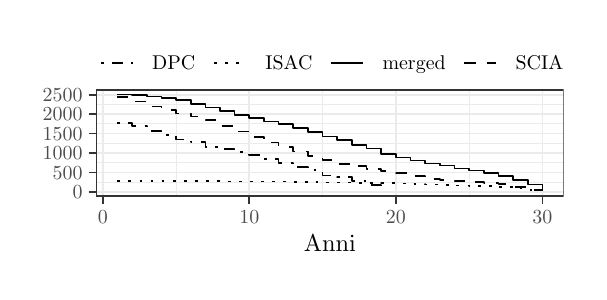
\begin{tikzpicture}[x=1pt,y=1pt]
\definecolor{fillColor}{RGB}{255,255,255}
\path[use as bounding box,fill=fillColor] (0,0) rectangle (199.17, 88.20);
\begin{scope}
\path[clip] (  0.00,  0.00) rectangle (199.17, 88.20);
\definecolor{drawColor}{RGB}{255,255,255}

\path[draw=drawColor,line width= 0.6pt,line join=round,line cap=round,fill=fillColor] (  0.00,  0.00) rectangle (199.17, 88.20);
\end{scope}
\begin{scope}
\path[clip] ( 24.75, 27.29) rectangle (193.67, 65.79);
\definecolor{fillColor}{RGB}{255,255,255}

\path[fill=fillColor] ( 24.75, 27.29) rectangle (193.67, 65.79);
\definecolor{drawColor}{gray}{0.92}

\path[draw=drawColor,line width= 0.3pt,line join=round] ( 24.75, 32.33) --
	(193.67, 32.33);

\path[draw=drawColor,line width= 0.3pt,line join=round] ( 24.75, 39.36) --
	(193.67, 39.36);

\path[draw=drawColor,line width= 0.3pt,line join=round] ( 24.75, 46.40) --
	(193.67, 46.40);

\path[draw=drawColor,line width= 0.3pt,line join=round] ( 24.75, 53.43) --
	(193.67, 53.43);

\path[draw=drawColor,line width= 0.3pt,line join=round] ( 24.75, 60.46) --
	(193.67, 60.46);

\path[draw=drawColor,line width= 0.3pt,line join=round] ( 53.61, 27.29) --
	( 53.61, 65.79);

\path[draw=drawColor,line width= 0.3pt,line join=round] (106.56, 27.29) --
	(106.56, 65.79);

\path[draw=drawColor,line width= 0.3pt,line join=round] (159.51, 27.29) --
	(159.51, 65.79);

\path[draw=drawColor,line width= 0.6pt,line join=round] ( 24.75, 28.81) --
	(193.67, 28.81);

\path[draw=drawColor,line width= 0.6pt,line join=round] ( 24.75, 35.85) --
	(193.67, 35.85);

\path[draw=drawColor,line width= 0.6pt,line join=round] ( 24.75, 42.88) --
	(193.67, 42.88);

\path[draw=drawColor,line width= 0.6pt,line join=round] ( 24.75, 49.91) --
	(193.67, 49.91);

\path[draw=drawColor,line width= 0.6pt,line join=round] ( 24.75, 56.95) --
	(193.67, 56.95);

\path[draw=drawColor,line width= 0.6pt,line join=round] ( 24.75, 63.98) --
	(193.67, 63.98);

\path[draw=drawColor,line width= 0.6pt,line join=round] ( 27.13, 27.29) --
	( 27.13, 65.79);

\path[draw=drawColor,line width= 0.6pt,line join=round] ( 80.09, 27.29) --
	( 80.09, 65.79);

\path[draw=drawColor,line width= 0.6pt,line join=round] (133.04, 27.29) --
	(133.04, 65.79);

\path[draw=drawColor,line width= 0.6pt,line join=round] (185.99, 27.29) --
	(185.99, 65.79);
\definecolor{drawColor}{RGB}{0,0,0}

\path[draw=drawColor,line width= 0.6pt,dash pattern=on 1pt off 3pt on 4pt off 3pt ,line join=round] ( 32.43, 53.80) --
	( 37.72, 53.80) --
	( 37.72, 52.61) --
	( 43.02, 52.61) --
	( 43.02, 50.93) --
	( 48.31, 50.93) --
	( 48.31, 49.34) --
	( 53.61, 49.34) --
	( 53.61, 47.73) --
	( 58.90, 47.73) --
	( 58.90, 46.83) --
	( 64.20, 46.83) --
	( 64.20, 45.06) --
	( 69.50, 45.06) --
	( 69.50, 44.46) --
	( 74.79, 44.46) --
	( 74.79, 43.19) --
	( 80.09, 43.19) --
	( 80.09, 42.15) --
	( 85.38, 42.15) --
	( 85.38, 40.83) --
	( 90.68, 40.83) --
	( 90.68, 39.35) --
	( 95.97, 39.35) --
	( 95.97, 37.77) --
	(101.27, 37.77) --
	(101.27, 36.69) --
	(106.56, 36.69) --
	(106.56, 34.83) --
	(111.86, 34.83) --
	(111.86, 34.22) --
	(117.15, 34.22) --
	(117.15, 32.77) --
	(122.45, 32.77) --
	(122.45, 31.37) --
	(127.74, 31.37) --
	(127.74, 29.53);

\path[draw=drawColor,line width= 0.6pt,dash pattern=on 1pt off 3pt ,line join=round] ( 32.43, 32.72) --
	( 37.72, 32.72) --
	( 37.72, 32.72) --
	( 43.02, 32.72) --
	( 43.02, 32.72) --
	( 48.31, 32.72) --
	( 48.31, 32.72) --
	( 53.61, 32.72) --
	( 53.61, 32.72) --
	( 58.90, 32.72) --
	( 58.90, 32.70) --
	( 64.20, 32.70) --
	( 64.20, 32.68) --
	( 69.50, 32.68) --
	( 69.50, 32.65) --
	( 74.79, 32.65) --
	( 74.79, 32.63) --
	( 80.09, 32.63) --
	( 80.09, 32.63) --
	( 85.38, 32.63) --
	( 85.38, 32.60) --
	( 90.68, 32.60) --
	( 90.68, 32.57) --
	( 95.97, 32.57) --
	( 95.97, 32.48) --
	(101.27, 32.48) --
	(101.27, 32.36) --
	(106.56, 32.36) --
	(106.56, 32.26) --
	(111.86, 32.26) --
	(111.86, 32.20) --
	(117.15, 32.20) --
	(117.15, 32.16) --
	(122.45, 32.16) --
	(122.45, 32.12) --
	(127.74, 32.12) --
	(127.74, 32.01) --
	(133.04, 32.01) --
	(133.04, 31.92) --
	(138.33, 31.92) --
	(138.33, 31.75) --
	(143.63, 31.75) --
	(143.63, 31.58) --
	(148.92, 31.58) --
	(148.92, 31.44) --
	(154.22, 31.44) --
	(154.22, 31.22) --
	(159.51, 31.22) --
	(159.51, 31.09) --
	(164.81, 31.09) --
	(164.81, 30.92) --
	(170.11, 30.92) --
	(170.11, 30.56) --
	(175.40, 30.56) --
	(175.40, 30.09) --
	(180.70, 30.09) --
	(180.70, 29.66) --
	(185.99, 29.66) --
	(185.99, 29.04);

\path[draw=drawColor,line width= 0.6pt,line join=round] ( 32.43, 64.04) --
	( 37.72, 64.04) --
	( 37.72, 63.94) --
	( 43.02, 63.94) --
	( 43.02, 63.39) --
	( 48.31, 63.39) --
	( 48.31, 62.74) --
	( 53.61, 62.74) --
	( 53.61, 62.01) --
	( 58.90, 62.01) --
	( 58.90, 60.72) --
	( 64.20, 60.72) --
	( 64.20, 59.34) --
	( 69.50, 59.34) --
	( 69.50, 58.04) --
	( 74.79, 58.04) --
	( 74.79, 56.64) --
	( 80.09, 56.64) --
	( 80.09, 55.48) --
	( 85.38, 55.48) --
	( 85.38, 54.29) --
	( 90.68, 54.29) --
	( 90.68, 53.29) --
	( 95.97, 53.29) --
	( 95.97, 51.95) --
	(101.27, 51.95) --
	(101.27, 50.46) --
	(106.56, 50.46) --
	(106.56, 48.90) --
	(111.86, 48.90) --
	(111.86, 47.54) --
	(117.15, 47.54) --
	(117.15, 45.85) --
	(122.45, 45.85) --
	(122.45, 44.50) --
	(127.74, 44.50) --
	(127.74, 42.65) --
	(133.04, 42.65) --
	(133.04, 41.26) --
	(138.33, 41.26) --
	(138.33, 40.24) --
	(143.63, 40.24) --
	(143.63, 39.11) --
	(148.92, 39.11) --
	(148.92, 38.35) --
	(154.22, 38.35) --
	(154.22, 37.28) --
	(159.51, 37.28) --
	(159.51, 36.59) --
	(164.81, 36.59) --
	(164.81, 35.62) --
	(170.11, 35.62) --
	(170.11, 34.57) --
	(175.40, 34.57) --
	(175.40, 33.24) --
	(180.70, 33.24) --
	(180.70, 31.50) --
	(185.99, 31.50) --
	(185.99, 29.63);

\path[draw=drawColor,line width= 0.6pt,dash pattern=on 4pt off 4pt ,line join=round] ( 32.43, 63.12) --
	( 37.72, 63.12) --
	( 37.72, 61.49) --
	( 43.02, 61.49) --
	( 43.02, 59.76) --
	( 48.31, 59.76) --
	( 48.31, 58.47) --
	( 53.61, 58.47) --
	( 53.61, 57.24) --
	( 58.90, 57.24) --
	( 58.90, 56.16) --
	( 64.20, 56.16) --
	( 64.20, 54.88) --
	( 69.50, 54.88) --
	( 69.50, 52.74) --
	( 74.79, 52.74) --
	( 74.79, 50.64) --
	( 80.09, 50.64) --
	( 80.09, 48.60) --
	( 85.38, 48.60) --
	( 85.38, 46.68) --
	( 90.68, 46.68) --
	( 90.68, 45.17) --
	( 95.97, 45.17) --
	( 95.97, 43.44) --
	(101.27, 43.44) --
	(101.27, 41.91) --
	(106.56, 41.91) --
	(106.56, 40.50) --
	(111.86, 40.50) --
	(111.86, 39.04) --
	(117.15, 39.04) --
	(117.15, 38.11) --
	(122.45, 38.11) --
	(122.45, 37.21) --
	(127.74, 37.21) --
	(127.74, 36.31) --
	(133.04, 36.31) --
	(133.04, 35.62) --
	(138.33, 35.62) --
	(138.33, 34.65) --
	(143.63, 34.65) --
	(143.63, 33.50) --
	(148.92, 33.50) --
	(148.92, 33.16) --
	(154.22, 33.16) --
	(154.22, 32.70) --
	(159.51, 32.70) --
	(159.51, 32.34) --
	(164.81, 32.34) --
	(164.81, 32.05) --
	(170.11, 32.05) --
	(170.11, 31.63) --
	(175.40, 31.63) --
	(175.40, 30.61) --
	(180.70, 30.61) --
	(180.70, 29.47) --
	(185.99, 29.47) --
	(185.99, 29.07);
\definecolor{drawColor}{gray}{0.20}

\path[draw=drawColor,line width= 0.6pt,line join=round,line cap=round] ( 24.75, 27.29) rectangle (193.67, 65.79);
\end{scope}
\begin{scope}
\path[clip] (  0.00,  0.00) rectangle (199.17, 88.20);
\definecolor{drawColor}{gray}{0.30}

\node[text=drawColor,anchor=base east,inner sep=0pt, outer sep=0pt, scale=  0.72] at ( 19.80, 26.35) {0};

\node[text=drawColor,anchor=base east,inner sep=0pt, outer sep=0pt, scale=  0.72] at ( 19.80, 33.38) {500};

\node[text=drawColor,anchor=base east,inner sep=0pt, outer sep=0pt, scale=  0.72] at ( 19.80, 40.42) {1000};

\node[text=drawColor,anchor=base east,inner sep=0pt, outer sep=0pt, scale=  0.72] at ( 19.80, 47.45) {1500};

\node[text=drawColor,anchor=base east,inner sep=0pt, outer sep=0pt, scale=  0.72] at ( 19.80, 54.48) {2000};

\node[text=drawColor,anchor=base east,inner sep=0pt, outer sep=0pt, scale=  0.72] at ( 19.80, 61.52) {2500};
\end{scope}
\begin{scope}
\path[clip] (  0.00,  0.00) rectangle (199.17, 88.20);
\definecolor{drawColor}{gray}{0.20}

\path[draw=drawColor,line width= 0.6pt,line join=round] ( 22.00, 28.81) --
	( 24.75, 28.81);

\path[draw=drawColor,line width= 0.6pt,line join=round] ( 22.00, 35.85) --
	( 24.75, 35.85);

\path[draw=drawColor,line width= 0.6pt,line join=round] ( 22.00, 42.88) --
	( 24.75, 42.88);

\path[draw=drawColor,line width= 0.6pt,line join=round] ( 22.00, 49.91) --
	( 24.75, 49.91);

\path[draw=drawColor,line width= 0.6pt,line join=round] ( 22.00, 56.95) --
	( 24.75, 56.95);

\path[draw=drawColor,line width= 0.6pt,line join=round] ( 22.00, 63.98) --
	( 24.75, 63.98);
\end{scope}
\begin{scope}
\path[clip] (  0.00,  0.00) rectangle (199.17, 88.20);
\definecolor{drawColor}{gray}{0.20}

\path[draw=drawColor,line width= 0.6pt,line join=round] ( 27.13, 24.54) --
	( 27.13, 27.29);

\path[draw=drawColor,line width= 0.6pt,line join=round] ( 80.09, 24.54) --
	( 80.09, 27.29);

\path[draw=drawColor,line width= 0.6pt,line join=round] (133.04, 24.54) --
	(133.04, 27.29);

\path[draw=drawColor,line width= 0.6pt,line join=round] (185.99, 24.54) --
	(185.99, 27.29);
\end{scope}
\begin{scope}
\path[clip] (  0.00,  0.00) rectangle (199.17, 88.20);
\definecolor{drawColor}{gray}{0.30}

\node[text=drawColor,anchor=base,inner sep=0pt, outer sep=0pt, scale=  0.72] at ( 27.13, 17.41) {0};

\node[text=drawColor,anchor=base,inner sep=0pt, outer sep=0pt, scale=  0.72] at ( 80.09, 17.41) {10};

\node[text=drawColor,anchor=base,inner sep=0pt, outer sep=0pt, scale=  0.72] at (133.04, 17.41) {20};

\node[text=drawColor,anchor=base,inner sep=0pt, outer sep=0pt, scale=  0.72] at (185.99, 17.41) {30};
\end{scope}
\begin{scope}
\path[clip] (  0.00,  0.00) rectangle (199.17, 88.20);
\definecolor{drawColor}{RGB}{0,0,0}

\node[text=drawColor,anchor=base,inner sep=0pt, outer sep=0pt, scale=  0.88] at (109.21,  7.21) {Anni};
\end{scope}
\begin{scope}
\path[clip] (  0.00,  0.00) rectangle (199.17, 88.20);
\definecolor{fillColor}{RGB}{255,255,255}

\path[fill=fillColor] ( 24.99, 76.79) rectangle (193.42, 82.70);
\end{scope}
\begin{scope}
\path[clip] (  0.00,  0.00) rectangle (199.17, 88.20);
\definecolor{fillColor}{RGB}{255,255,255}

\path[fill=fillColor] ( 24.99, 68.25) rectangle ( 39.45, 82.70);
\end{scope}
\begin{scope}
\path[clip] (  0.00,  0.00) rectangle (199.17, 88.20);
\definecolor{drawColor}{RGB}{0,0,0}

\path[draw=drawColor,line width= 0.6pt,dash pattern=on 1pt off 3pt on 4pt off 3pt ,line join=round] ( 26.44, 75.48) -- ( 38.00, 75.48);
\end{scope}
\begin{scope}
\path[clip] (  0.00,  0.00) rectangle (199.17, 88.20);
\definecolor{fillColor}{RGB}{255,255,255}

\path[fill=fillColor] ( 65.94, 68.25) rectangle ( 80.39, 82.70);
\end{scope}
\begin{scope}
\path[clip] (  0.00,  0.00) rectangle (199.17, 88.20);
\definecolor{drawColor}{RGB}{0,0,0}

\path[draw=drawColor,line width= 0.6pt,dash pattern=on 1pt off 3pt ,line join=round] ( 67.39, 75.48) -- ( 78.95, 75.48);
\end{scope}
\begin{scope}
\path[clip] (  0.00,  0.00) rectangle (199.17, 88.20);
\definecolor{fillColor}{RGB}{255,255,255}

\path[fill=fillColor] (108.28, 68.25) rectangle (122.73, 82.70);
\end{scope}
\begin{scope}
\path[clip] (  0.00,  0.00) rectangle (199.17, 88.20);
\definecolor{drawColor}{RGB}{0,0,0}

\path[draw=drawColor,line width= 0.6pt,line join=round] (109.72, 75.48) -- (121.28, 75.48);
\end{scope}
\begin{scope}
\path[clip] (  0.00,  0.00) rectangle (199.17, 88.20);
\definecolor{fillColor}{RGB}{255,255,255}

\path[fill=fillColor] (156.39, 68.25) rectangle (170.84, 82.70);
\end{scope}
\begin{scope}
\path[clip] (  0.00,  0.00) rectangle (199.17, 88.20);
\definecolor{drawColor}{RGB}{0,0,0}

\path[draw=drawColor,line width= 0.6pt,dash pattern=on 4pt off 4pt ,line join=round] (157.84, 75.48) -- (169.40, 75.48);
\end{scope}
\begin{scope}
\path[clip] (  0.00,  0.00) rectangle (199.17, 88.20);
\definecolor{drawColor}{RGB}{0,0,0}

\node[text=drawColor,anchor=base west,inner sep=0pt, outer sep=0pt, scale=  0.72] at ( 44.95, 73.01) {DPC};
\end{scope}
\begin{scope}
\path[clip] (  0.00,  0.00) rectangle (199.17, 88.20);
\definecolor{drawColor}{RGB}{0,0,0}

\node[text=drawColor,anchor=base west,inner sep=0pt, outer sep=0pt, scale=  0.72] at ( 85.89, 73.01) {ISAC};
\end{scope}
\begin{scope}
\path[clip] (  0.00,  0.00) rectangle (199.17, 88.20);
\definecolor{drawColor}{RGB}{0,0,0}

\node[text=drawColor,anchor=base west,inner sep=0pt, outer sep=0pt, scale=  0.72] at (128.23, 73.01) {merged};
\end{scope}
\begin{scope}
\path[clip] (  0.00,  0.00) rectangle (199.17, 88.20);
\definecolor{drawColor}{RGB}{0,0,0}

\node[text=drawColor,anchor=base west,inner sep=0pt, outer sep=0pt, scale=  0.72] at (176.34, 73.01) {SCIA};
\end{scope}
\end{tikzpicture}

  \caption{Disponibilità di serie con un numero minimo di anni a seconda del dataset.}\label{fig:merged-improvements}
\end{figure}
